\documentclass[12pt]{extarticle}
%%%%%%%%%%%%%%% PACKAGES %%%%%%%%%%%%%%%
\usepackage{titleps}
\usepackage{url}
\usepackage{amsmath}
\usepackage{cancel}
\usepackage{amsfonts}
\usepackage{booktabs}
\usepackage{amssymb}
\usepackage{mathtools}
\usepackage{graphicx}
\usepackage{subfig}
\usepackage[dvipsnames]{xcolor}
\usepackage[colorlinks]{hyperref}
\usepackage{geometry}
\geometry{
    a4paper,
    left=19mm,
    right=19mm,
    top=20mm,
    bottom=25mm
}
% Define dark and mid color

\definecolor{Sepia}{HTML}{704214}
\definecolor{RedViolet}{HTML}{C71585}

\hypersetup{
	colorlinks=true,
	linkcolor=Golden,
    linkcolor=Golden,
    filecolor=Golden,
    citecolor = Golden,
    urlcolor=Golden, % change this to your desired color
}

% Mix lighter shade

\colorlet{LightSepia1}{Sepia!80!yellow}
\colorlet{LightSepia2}{Sepia!70!orange}
\colorlet{DarkGolden}{RedViolet!30!yellow!70!Maroon!70!Brown}
\colorlet{Golden}{RedViolet!30!yellow!70!pink!90!Brown}
\colorlet{DDarkGolden}{RedViolet!20!yellow!70!Maroon!70!Black!65!Brown}

%%%%%%%%%%%%%%%%%%%%%%%%%%%%%%%%%%%%%%%%
%%%%%%%%%%%%%%% FONT %%%%%%%%%%%%%%%%%%%
\usepackage[T1]{fontenc}
\usepackage{charter}

\def\primarycolor{DarkGolden}
\def\secondarycolor{Golden}
%%%%%%%%%%%%%%%%%%%%%%%%%%%%%%%%%%%%%%%%
%%%%%%%%%%%%%%% HEADER %%%%%%%%%%%%%%%%%
\usepackage{fancyhdr}
\let\oldheadrule\headrule
\renewcommand{\headrule}{\color{\secondarycolor}\oldheadrule}
\renewcommand{\headrulewidth}{0.7pt}
\pagestyle{fancy}
\fancyhead{}\fancyfoot{}
\fancyhead[L]{\scshape \large \color{\primarycolor}{\fontfamily{qpl}\selectfont
Amirreza "Farnam" Taheri \\
Student ID: 4021300198003
}}
\fancyhead[R]{\color{\secondarycolor}}
\fancyfoot[C]{\textcolor{\primarycolor}{(\thepage)}}
\setlength{\headheight}{1cm}

\fancypagestyle{headerpage}{
    \fancyhf{} % Clear header and footer
    \renewcommand{\headrulewidth}{0pt} % Remove header rule
    \renewcommand{\footrulewidth}{0pt} % Remove footer rule
    \fancyhead[R]{} % Remove the line that displays "Course Name (Course Code)" in the header page
}

%%%%%%%%%%%%%%%%%%%%%%%%%%%%%%%%%%%%%%%%
%%%%%%%%%%%%%%% COMMANDS %%%%%%%%%%%%%%%
% \newcommand{\norm}[1]{\lVert#1\rVert}
% \newcommand{\inner}[1]{\langle#1\rangle}
\newcommand{\problem}[1]{
    \subsection*{\textcolor{\secondarycolor}{#1}}
    \addcontentsline{toc}{subsection}{\protect\numberline{}#1}
}
\newcommand{\partof}[1]{
    \subsubsection*{\textcolor{\secondarycolor}{(#1)}}
    \addcontentsline{toc}{subsubsection}{\protect\numberline{}#1}
}
\newcommand{\imp}{\implies}
\newcommand{\rond}[2]{\frac{\partial #1}{\partial #2}}
\newcommand{\drond}[2]{\dfrac{\partial #1}{\partial #2}}
\newcommand{\norm}[1]{\lvert#1\rvert}
\newcommand{\expec}[1]{\mathbb{E}\left(#1\right)}
\newcommand{\var}[1]{\mathrm{Var}\left(#1\right)}
\newcommand{\cov}[1]{\mathrm{Cov}\left(#1\right)}
\newcommand{\prob}[1]{\mathbb{P}\left(#1\right)}
\newcommand{\ones}{$\star$}
\newcommand{\twos}{$\star\star$}
\newcommand{\threes}{$\star\star\star$}
\newcommand{\fours}{$\star\star\star\star$}
%%%%%%%%%%%%%%%%%%%%%%%%%%%%%%%%%%%%%%%%
%%%%%%%%%%%%%%% BODY %%%%%%%%%%%%%%%%%%%
\linespread{1.4}
\color{DDarkGolden}
\begin{document}
\setlength{\abovedisplayskip}{6pt}
\setlength{\belowdisplayskip}{6pt}
\setlength{\abovedisplayshortskip}{0pt}
\setlength{\belowdisplayshortskip}{0pt}
%%%%%%%%%%%%%%% CONTENT %%%%%%%%%%%%%%%%
\thispagestyle{headerpage} % Apply custom header style to this page only
\begin{center}
    \vspace*{1.5cm}
    {\Huge\bfseries\color{\primarycolor}{\fontfamily{qpl}\selectfont Exercise 8}} \\
    \vspace{3cm}
    
\includegraphics[width=6cm]{teias.png} \\ % Replace "university_logo.png" with the actual filename of your university logo
    \vspace{2cm}
    {\Large\color{\primarycolor}{\fontfamily{qpl}\selectfont Amirreza "Farnam" Taheri}} \\
    {\large\color{\primarycolor}{Student ID: 4021300198003}} \\
    \vspace{3cm}
    {\large\bfseries\color{\secondarycolor}{Macroeconomics I}} \\
    \vspace{1cm}
    {\large\color{\secondarycolor}{Instructor: Prof. Hosein Joshaghani}} \\
    \vspace{3cm}
    {\large\color{\secondarycolor}{May 11, 2024}} % Replace with the actual date or semester information
\end{center}
\newpage % Add a page break after the header page

%%%%%%%%%%%%%%% CONTENT %%%%%%%%%%%%%%%%
\pagestyle{fancy} % Apply fancy header to the remaining pages
\fancyhead[R]{\color{\secondarycolor} Problemset 8} % Display "Problemset #no" in the header of the remaining pages
%%%%%%%%%%%%%%%%%%%%%%%%%%%%%%%%%%%%%%%%
%%%%%%%%%%%%%%%%%%%%%%%%%%%%%%%%%%%%%%%%
\problem{\textsc{RBC: Extensions}}
Consider an economy similar to the one you see in project 1. Assume, however, that the household preferences
takes the form

$$u(c_t,N_t) = \frac{\left(C_t v(1 - N_t)\right)^{1-\sigma} - 1}{1 - \sigma}$$
where
$$v(1 - N_t) = \exp\left(\frac{\theta(1 - N_t)^{1-\zeta} - 1}{1 - \zeta}\right)$$\\
Assume:
\begin{align}
    \alpha = 1/3, \;\rho_A = 0.95, \;\delta = 0.025, \;\beta = 0.99,\; \theta = 0.5,\; \sigma = \zeta = 2.
\end{align}\\
Find the set of FOCs describing the competitive equilibrium of the system, and use Dynare to plot IRFs for
$Y, c, N, I, w, r$. Compare these with your results for the case of quasi-linear utility representation function.
Intuitively explain the differences between them. \newpage

\partof{Household's Problem}
The representative household maximizes its lifetime utility function subject to it budget constraint:
   \begin{align}
    \underset{c_t,k_{t+1}, N_t}{\max}\quad U &= \mathbb{E}_t \left[ \sum_{i=0}^{\infty} \beta^{t} \left(\frac{\left(c_t\;v(1 - N_t)\right)^{1-\sigma} - 1}{1 - \sigma} \right) \right],\\
    \text{where:}\quad v(1 - N_t) &= \exp\left(\frac{\theta(1 - N_t)^{1-\zeta} - 1}{1 - \zeta}\right),\\
    \text{s.t.  }\quad c_t + k_{t+1} &\leq w_t N_t + (1 + R_t - \delta) k_t + \Pi_t.
   \end{align}\\
The Lagrangian for the houehold's problem is:
\begin{equation}
    \mathcal{L}= \mathbb{E}_t\sum_{i=0}^{\infty} \beta^{t} \left[  \left(\frac{\left(c_t\;v(1 - N_t)\right)^{1-\sigma} - 1}{1 - \sigma} \right)
    -\mu_{t}\left( c_t + k_{t+1} - w_t N_t - (1 + R_t - \delta) k_t -\Pi_t \right)\right].
\end{equation} \\\\
The FOCs are:

\begin{align}
    \frac{\partial \mathcal{L}}{\partial c_t} &= 0 \implies c_t^{-\sigma} v(1-N_t)^{1-\sigma} = \mu_t,\\
    \frac{\partial \mathcal{L}}{\partial N_t} &= 0 \implies -c_t^{1-\sigma}\;v'(1-N_t)\;v(1-N_t)^{-\sigma} = \mu_t w_t, \\
    \frac{\partial \mathcal{L}}{\partial k_{t+1}} &= 0 \implies \mu_t = \beta \mathbb{E}_t \left[ \mu_{t+1} (1+R_{t+1}-\delta) \right],\\
    \frac{\partial \mathcal{L}}{\partial \mu_t} &= 0 \implies c_t + k_{t+1} = w_t N_t + (1+R_t-\delta) k_t + \Pi_t .
\end{align}\\
We had: 
$$v(1-N_t) = \exp\left(\frac{\theta(1-N_t)^{1-\zeta}-1}{1-\zeta}\right)$$\\
Which imlplies:
$$v'(1-N_t) = -\theta (1-N_t)^{-\zeta}\exp\left(\frac{\theta(1-N_t)^{1-\zeta}-1}{1-\zeta}\right)$$\\
\newpage
Substituting into FOCs, we get the following conditions:
\setcounter{equation}{0}
\renewcommand{\theequation}{\roman{equation}}
\begin{align}
    \frac{\partial \mathcal{L}}{\partial c_t} &= 0 \implies c_t^{-\sigma}\exp\left(\frac{\theta(1-N_t)^{1-\zeta}-1}{1-\zeta}\right)^{1-\sigma} = \mu_t, \label{equation:eq1}\\
    \frac{\partial \mathcal{L}}{\partial N_t} &= 0 \implies c_t^{1-\sigma}\;\theta (1-N_t)^{-\zeta}\exp\left(\frac{\theta(1-N_t)^{1-\zeta}-1}{1-\zeta}\right)^{-\sigma+1} = \mu_t w_t, \label{equation:eq2}\\
    \frac{\partial \mathcal{L}}{\partial k_{t+1}} &= 0 \implies \mu_t = \beta \mathbb{E}_t \left[ \mu_{t+1} (1+R_{t+1}-\delta) \right], \label{equation:eq3}\\
    \frac{\partial \mathcal{L}}{\partial \mu_t} &= 0 \implies c_t + k_{t+1} = w_t N_t + (1+R_t-\delta) k_t + \Pi_t \label{equation:eq4}.
\end{align}\\
From \href{equation:eq1}{(i)}, \href{equation:eq2}{(ii)}, we get intertemporal optimality condition:\\
\begin{align}
    c_t\;\theta (1-N_t)^{-\zeta} =  w_t, \label{equation:eq5}
\end{align}\\
From \href{equation:eq1}{(i)}, \href{equation:eq3}{(iii)}, we get intratemporal omptimality condition:\\
\begin{align}
    c_t^{-\sigma}{\exp\left({\theta(1-N_t)^{1-\zeta}-1}\right)^{1-\sigma}} = \beta \mathbb{E}_t \left[  c_{t+1}^{-\sigma}{\exp\left({\theta(1-N_{t+1})^{1-\zeta}-1}\right)^{1-\sigma}} (1+R_{t+1}-\delta) \right]
\end{align}

\newpage
%%%%%%%%%%%%%%%%%%%%%%%%%%%%%%%%%%%%%%%%
\partof{Firm's Problem}
\setcounter{equation}{0}
\renewcommand{\theequation}{\arabic{equation}}
The firm's technology is described by the production function:
    \begin{equation}
    Y_t = z_t k_t^{\alpha} N_t^{1-\alpha}
   \end{equation} \\
The technology follows an $AR1$ process:
    \begin{equation}
    \log(z_{t+1}) = \rho \log(z_t) + \epsilon_t, \quad \epsilon_t \sim IID
   \end{equation} \\
Firm wants to maximize its profit:
\begin{equation}
    \max\quad \Pi_t = z_t k_t^{\alpha} N_t^{1-\alpha} - w_t N_t - R_t k_t 
   \end{equation}\\
\setcounter{equation}{6}
\renewcommand{\theequation}{\roman{equation}}
The optimality conditions are:
   \begin{align}
        MP_L &= (1-\alpha) z_t k_t^{\alpha} N_t^{-\alpha} = w_t\\
        MP_K &= \alpha\; z_t k_t^{\alpha-1} N_t^{1-\alpha} = R_t
    \end{align}\\\\
The structural equations of the economy are:
\begin{align}
    \textsc{(LNS,\;Market Clearing)}&\qquad c_t + k_{t+1} = w_t N_t + (1 + R_t - \delta) k_t + \Pi_t\\
    \textsc{(Production of Economy)}&\qquad \qquad \;\;\;Y_t = z_t k_t^{\alpha} N_t^{1-\alpha}
\end{align}
    
\newpage
%%%%%%%%%%%%%%%%%%%%%%%%%%%%%%%%%%%%%%%%
\partof{The Steady State}
\setcounter{equation}{0}
In the steady state we have no shock and zero profit $(\Pi=0,\;z=1)$.
Also the sytem parameters has no dynamic. So the equations are:\\
$$\textbf{Supply:}$$
\begin{align}
    c\;\theta (1-N)^{-\zeta}(1-\sigma) &=  w, \label{equation:eq_1}\\
    c^{-\sigma} &= \beta  \left[ (1+R-\delta) \right]. \label{equation:eq_2}
\end{align}\\
$$\textbf{Demand:}$$
\begin{align}
    (1-\alpha)\; k^{\alpha} N^{-\alpha} &= w, \label{equation:eq_3}\\
    \alpha\; k^{\alpha-1} N^{1-\alpha} &= R. \label{equation:eq_4}
\end{align}\\
$$\textbf{Structural equations:}$$
\begin{align}
    Y &= C + I, \label{equation:eq_5}\\
    Y &= k^{\alpha} N^{1-\alpha}\label{equation:eq_6}\\
    \log(z) &= \rho \log(z) \label{equation:eq_7}\\
    k&= k (1-\delta) + i\label{equation:eq_8}
\end{align}\\
\newpage
%%%%%%%%%%%%%%%%%%%%%%%%%%%%%%%%%%%%%%%%
\partof{IRF Comparison}
\begin{figure}[htpb]%
    \centering
    \subfloat[\centering Quasi-Linear Utility]{{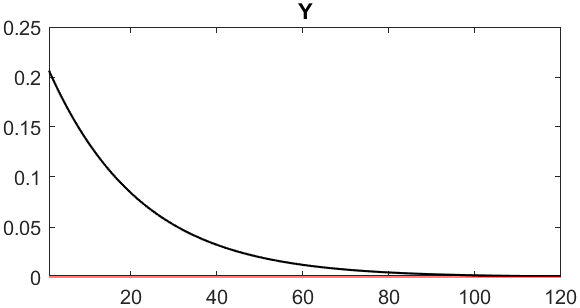
\includegraphics[width=8cm]{Y_1} }}%
    \qquad
    \subfloat[\centering Non-Seperable Utility]{{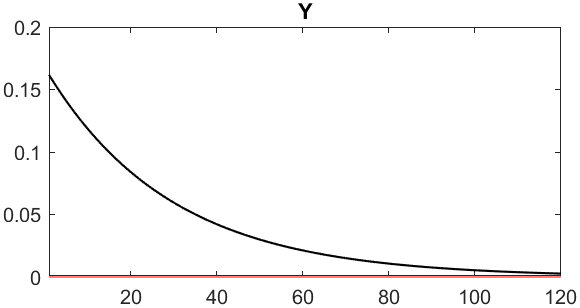
\includegraphics[width=8cm]{Y_2} }}%
    \caption{Output's IRF Comparison}%
    \label{fig:Output}%
\end{figure}
\vspace{0.5cm}
\begin{figure}[htpb]%
    \centering
    \subfloat[\centering Quasi-Linear Utility]{{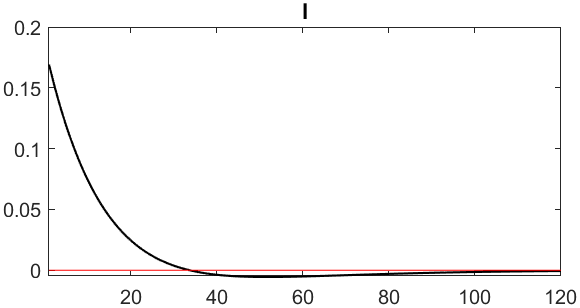
\includegraphics[width=8cm]{I_1} }}%
    \qquad
    \subfloat[\centering Non-Seperable Utility]{{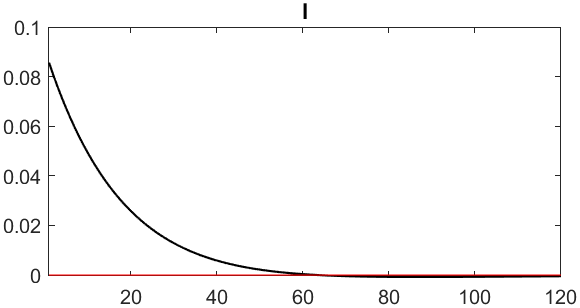
\includegraphics[width=8cm]{I_2} }}%
    \caption{Investment's IRF Comparison}%
    \label{fig:Investment}%
\end{figure}
\vspace{0.5cm}
\begin{figure}[h!]%
    \centering
    \subfloat[\centering Quasi-Linear Utility]{{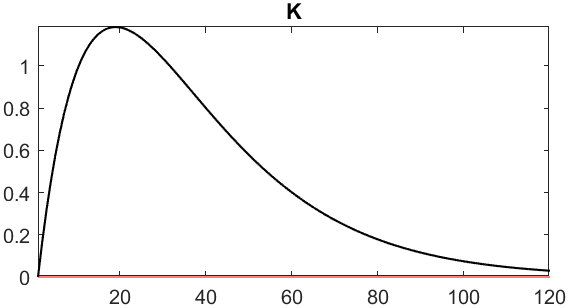
\includegraphics[width=8cm]{K_1} }}%
    \qquad
    \subfloat[\centering Non-Seperable Utility]{{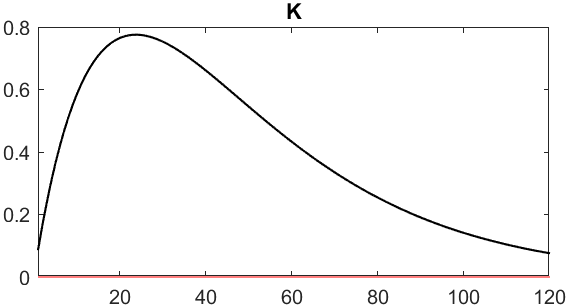
\includegraphics[width=8cm]{K_2} }}%
    \caption{Capital's IRF Comparison}%
    \label{fig:Capital}%
\end{figure}
\newpage
\begin{figure}[h!]%
    \centering
    \subfloat[\centering Quasi-Linear Utility]{{\includegraphics[width=8cm]{Rk_1} }}%
    \qquad
    \subfloat[\centering Non-Seperable Utility]{{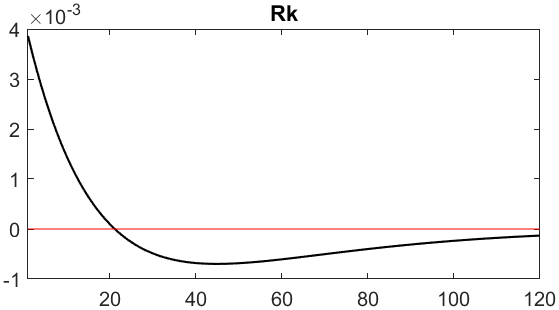
\includegraphics[width=8cm]{Rk_2} }}%
    \caption{Interest Rate's IRF Comparison}%
    \label{fig:Interest Rate}%
\end{figure}
\vspace{0.5cm}
\begin{figure}[htpb]%
    \centering
    \subfloat[\centering Quasi-Linear Utility]{{\includegraphics[width=8cm]{w_1} }}%
    \qquad
    \subfloat[\centering Non-Seperable Utility]{{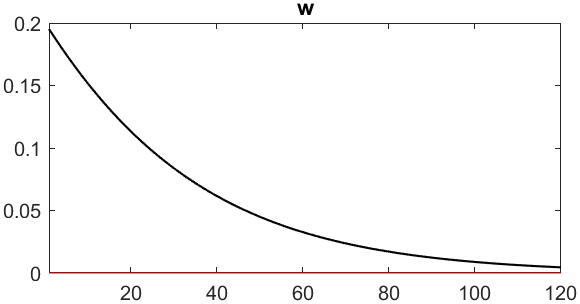
\includegraphics[width=8cm]{w_2} }}%
    \caption{Technology's IRF Comparison}%
    \label{fig:Wage}%
\end{figure}
\vspace{0.5cm}
\begin{figure}[h!]%
    \centering
    \subfloat[\centering Quasi-Linear Utility]{{\includegraphics[width=8cm]{w_1} }}%
    \qquad
    \subfloat[\centering Non-Seperable Utility]{{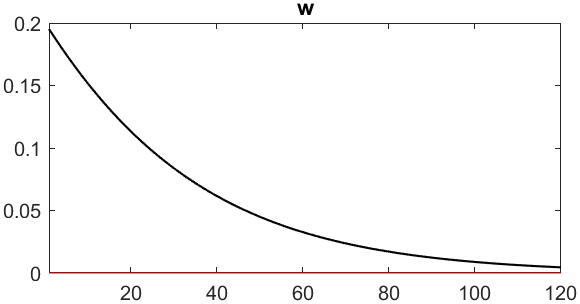
\includegraphics[width=8cm]{w_2} }}%
    \caption{Wage's IRF Comparison}%
    \label{fig:Technology}%
\end{figure}
\newpage
\begin{figure}[htpb]%
    \centering
    \subfloat[\centering Quasi-Linear Utility]{{\includegraphics[width=8cm]{c_1} }}%
    \qquad
    \subfloat[\centering Non-Seperable Utility]{{\includegraphics[width=8cm]{c_2} }}%
    \caption{Consumption's IRF Comparison}%
    \label{fig:Consumption}%
\end{figure}
\vspace{0.5cm}
\begin{figure}[h!]%
    \centering
    \subfloat[\centering Quasi-Linear Utility]{{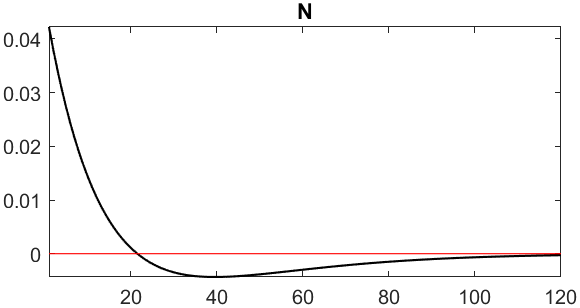
\includegraphics[width=8cm]{N_1} }}%
    \qquad
    \subfloat[\centering Non-Seperable Utility]{{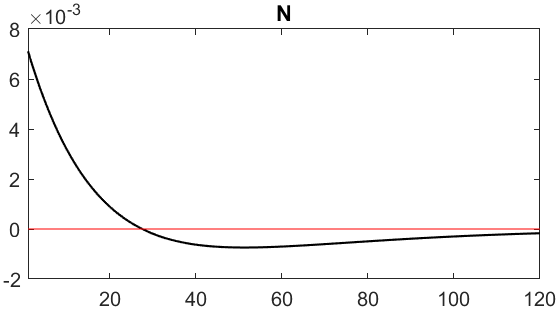
\includegraphics[width=8cm]{N_2} }}%
    \caption{Labor's IRF Comparison}
    \label{fig:Labor}
\end{figure}

\begin{center}
    \large\textbf{ To open the Dynare script for this problem:\\\vspace*{0.5cm}
    \textbf{\href{run:Farnam_RBC_SSmodel}{Click here to open the code utilizing steady\_state\_model method}}}.\\\vspace*{0.3cm}
    \large\textbf{Or alternatively,}\\\vspace*{0.3cm}
    \textbf{\href{run:Farnam_RBC_initval}{Click here to open the code utilizing initval method}}.\\
\end{center}
\newpage
%%%%%%%%%%%%%%%%%%%%%%%%%%%%%%%%%%%%%%%%
%%%%%%%%%%%%%%%%%%%%%%%%%%%%%%%%%%%%%%%%
\renewcommand{\theequation}{\arabic{equation}}
\setcounter{equation}{0}
\problem{\textsc{Introduction to Dynamic Programming}}
Your utility representation function is
\begin{align}
    u(c) = \frac{c^{1-\sigma}}{1-\sigma}. \label{equation:dp1}
\end{align}
Initially you are endowed with 1 unit of cake. Your problem is choosing the optimal consumption path to
maximize the present value of the sum of your utility gains from eating cake. Formally, this would be
\begin{align}
    \max_{c_t,x_{t+1}} \sum_{t=0}^\infty \beta^t u(c_t), \label{equation:dp2}
\end{align}
subject to
\begin{align}
    x_{t+1} \leq x_t - c_t \quad \text{and} \quad 0 \leq c_t \leq x_t, \label{equation:dp3}
\end{align}
with $x_0 = 1$.
\newpage
%%%%%%%%%%%%%%%%%%%%%%%%%%%%%%%%%%%%%%%%
\setcounter{equation}{0}
\problem{1.  Bellman Equation}
Write the Bellman equation of this problem.\\\\\\\\
The problem is to:
\begin{align}
    \max_{c_t, x_{t+1}} \sum_{t=0}^{\infty} \beta^t u(c_t), \label{equation:dp_1}
\end{align}
subject to the constraint:
\begin{align}
    x_{t+1} \leq x_t - c_t \quad \text{and} \quad 0 \leq c_t \leq x_t, \label{equation:dp_2}
\end{align}
with the initial condition $x_0 = 1$.\\\\\\
The problem is equivalent to finding the value function $v(x_t)$ that satisfies:
\begin{align}
    v(x_t) = \max_{c_t \in [0, x_t]} \left\{ u(c_t) + \beta v(x_{t+1}) \right\}, \label{equation:dp_3}
\end{align}\\
where $u(c_t) = \frac{c_t^{1-\sigma}}{1-\sigma}$, and the constraint $c_t = x_t - x_{t+1}$ holds, with $x_0 = 1$ .\\\\
Thus, the Bellman equation is:
\begin{align}
    v(x_t) = \max_{x_{t+1} \in [0, x]} \left\{ \frac{(x_t - x_{t+1})^{1-\sigma}}{1-\sigma} + \beta v(x_{t+1}) \right\}. \label{equation:dp_4}
\end{align}\\

\newpage
%%%%%%%%%%%%%%%%%%%%%%%%%%%%%%%%%%%%%%%%
\problem{2. Value Function}
\setcounter{equation}{0}
\renewcommand{\theequation}{\arabic{equation}}
Show that the value function of this problem is
$$
v^*(x_t) = \left(1 - \beta^{\frac{1}{\sigma}}\right)^{-\sigma} u(x_t).
$$\\\\\\
%%%%%%%%%%%%%%%%%%%%%%%%%%%%%%%%%%%%%%%%
To show that the value function is
\begin{align}
    v^*(x_t) = \left(1 - \beta^{\frac{1}{\sigma}}\right)^{-\sigma} u(x_{t+1}), \label{equation:dp_2_2_1}
\end{align}
we need to verify that this function satisfies the Bellman equation.\\\\
Substituting \href{equation:dp_2_2_1}{$v^*(x_t)$} into the \href{equation:eq1}{Bellman equation}, we get:
\begin{align}
    \max_{x_{t+1} \in [0, x]} \left\{u(x_t-x_{t+1}) + \beta \left(1 - \beta^{\frac{1}{\sigma}}\right)^{-\sigma}u(x_{t+1}) \right\} \overset{?}{=}  \left(1 - \beta^{\frac{1}{\sigma}}\right)^{-\sigma} u(x_{t+1}). \label{equation:dp_2_2_2}
\end{align}\\\\
Taking the FOC from the \href{equation:dp_2_2}{Bellman equation} yields:\\
\begin{align*}
    \dfrac{d}{d x_{t+1}}v(x_t) &= \dfrac{d}{d x_{t+1}} \left( u(x_t-x_{t+1}) + \beta \left(1 - \beta^{\frac{1}{\sigma}}\right)^{-\sigma}u(x_{t+1}) \right)\\
    & =  -u'(x_t-x_{t+1}) + \beta \left(1 - \beta^{\frac{1}{\sigma}}\right)^{-\sigma}u'(x_{t+1}) = 0\\
    \implies \left(\dfrac{x_t-x_{t+1}}{x_{t+1}}\right)^{-\sigma} &= \beta \left(1 - \beta^{\frac{1}{\sigma}}\right)^{-\sigma}\\
    \implies \qquad \dfrac{x_t}{\beta^{-\frac{1}{\sigma}}\left(1 - \beta^{\frac{1}{\sigma}}\right)+1} &= x_{t+1}
\end{align*}\\
Since $x_{t+1} \in [0, x_t]$, we have interior solution.\\\\
Substituting  $x_{t+1} = \dfrac{x_t}{\beta^{-\frac{1}{\sigma}}\left(1 - \beta^{\frac{1}{\sigma}}\right)+1}$
into the LHS of Bellman equation, we will reach the \href{equation:dp_2_2_1}{proposed value function}
\newpage
%%%%%%%%%%%%%%%%%%%%%%%%%%%%%%%%%%%%%%%%
\problem{3. Value Function Iteration}
Use value function iteration to numerically solve for $v^*$. Compare your results.($\sigma = 3,\;\beta = 0.98$)\\\\\\

\begin{figure}[htpb]
    \centering
    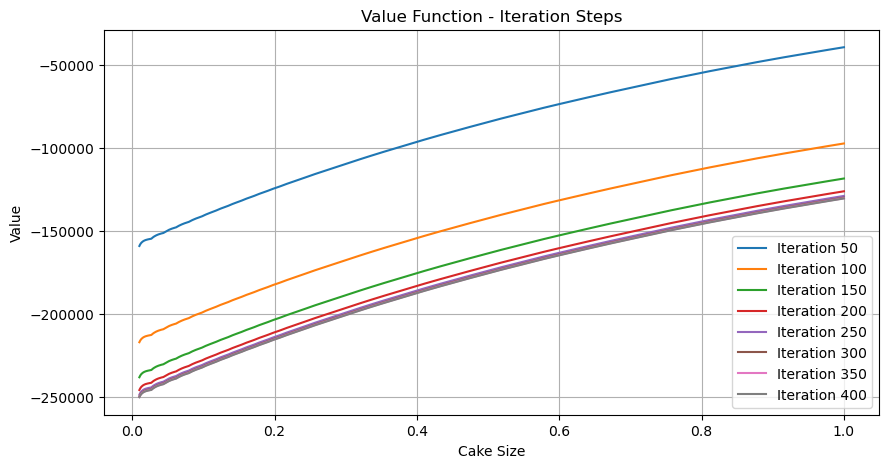
\includegraphics[scale=0.5]{iter.png}
    \caption{Iteration Plot}
    \label{fig:fig9}
\end{figure}
\begin{figure}[htpb]
    \centering
    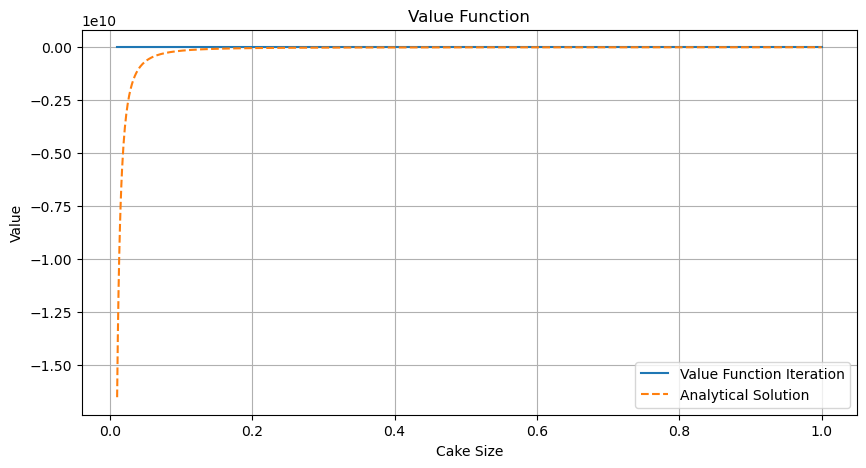
\includegraphics[scale=0.5]{value.png}
    \caption{Anaytical vs. Numerical Comparison}
    \label{fig:fig10}
\end{figure}
\begin{center}
    \large\textbf{ To open the .ipynb file for this problem \textbf{\href{run:DP2.ipynb}{Click Here!}}}
\end{center}
%%%%%%%%%%%%%%%%%%%%%%%%%%%%%%%%%%%%%%%%
%%%%%%%%%%%%%%%%%%%%%%%%%%%%%%%%%%%%%%%%
\end{document}

import numpy as np

sigma = 3
beta = 0.98
x_max = 1
n_grid = 100
x_grid = np.linspace(0, x_max, n_grid)
v_grid = np.zeros((n_grid,))

def u(c):
    return c**(1-sigma)/(1-sigma)

def v(x, v_grid):
    c_opt = np.argmax([u(c) + beta*v_grid[i] for i, c in enumerate(x_grid) if c <= x])
    return u(x_grid[c_opt]) + beta*v_grid[c_opt]

for i in range(100):
    v_grid = np.array([v(x, v_grid) for x in x_grid])

v_star = (1 - beta**(1/sigma))**(-sigma)*u(x_grid)